\chapter[Анализ состояния проблемы. Постановка задачи исследования]{%
  АНАЛИЗ СОСТОЯНИЯ ПРОБЛЕМЫ. \hspace{2cm}
  ПОСТАНОВКА ЗАДАЧИ ИССЛЕДОВАНИЯ
}

\section{История развития теории идентификации систем}

Начало идентификации систем, как предмета построения математических моделей на основе наблюдений,
связано с работами~\cite{gauss_1809, gauss_1810, gauss_1821} К.~Гаусса,
в которых он разработал метод наименьших квадратов и использовал его для предсказания
траектории движения планет.
Впоследствии МНК нашёл применение во множестве других приложений,
в том числе для построения математических моделей управляемых объектов,
используемых в автоматизации.
Существенный вклад в развитие МНК внесли
П.~Лаплас~\cite{laplace_1812},
П.~Чебышев~\cite{chebyshev_1859},
А.~Марков~\cite{markov_1898},
А.~Эйткен~\cite{aitken_1935},
А.~Колмогоров~\cite{kolmogorov_1946} и
С.~Рао~\cite{rao_1946}.
Системное изложение этого метода представлено, например, в монографии Ю.~Линника~\cite{linnik62}.

Большая часть ранних работ по идентификации систем была сделана специалистами в области статистики,
эконометрики и образовала область под названием статистическое оценивание.
Следует отметить, что область приложений этих методов была ограничена чаще всего скалярными системами.
В 1960 году Р.~Калман представил описание управляемой системы в виде пространства состояний,
что позволяло работать и с многомерными системами,
и заложил основы для оптимальной фильтрации и оптимального управления,
основывавшихся на данном типе описания.

Методы идентификации систем для задач управления были разработаны в 1965 году в работах
Б.~Хо и Р.~Калмана~\cite{ho_1965}, К.~Острёма и Т.~Болина~\cite{astrom_1965}.
Работа Хо и Калмана посвящена поиску модели изучаемого объекта в пространстве состояний,
имеющей наименьший порядок вектора состояний,
на основе информации об импульсной переходной характеристике.
Данная задача, но уже при наличии реализаций случайного процесса, где формируется марковская модель,
была решена в 70-х годах в работах П.~Форре~\cite{faurre_1973} и Х.~Акайка~\cite{akaike_1974}.
Эти работы заложили создание метода подпространства в начале 90-х.

Работа Острёма и Болина представила для сообщества специалистов по идентификации метод
максимального правдоподобия, который был разработан специалистами по временным рядам для
оценивания параметров моделей в виде разностных уравнений~\cite{koopmans_1950}.
Эти модели, которые известны в статистической литературе как ARMA
(авторегрессионное скользящее среднее) и
ARMAX (авторегрессионное скользящее среднее со входом), позднее,
образовали основу для создания метода ошибки предсказания.
В 1970-х годах этот метод стал доминировать в теории и, что более важно, в приложениях идентификации.

Большая часть исследовательской активности того времени фокусировалась на проблемах идентификации
многомерных и замкнутых систем.
Ключевой задачей для этих двух классов систем являлось найти условия для эксперимента и
способы параметризации проблемы, при которых найденная модель приблизится к единственно точному
описанию реальной системы.

В конце 1970-х годов была сделана первая попытка рассмотреть идентификацию систем как
теорию аппроксимации, в которой стоит задача наилучшей возможной аппроксимации реальной системы
внутри данного класса моделей~\cite{ljung_1976, anderson_1978, ljung_1979}.
Таким образом, преобладающая точка зрения среди специалистов по идентификации сменилась с
поиска описания истинной системы на поиск описания наилучшей возможной аппроксимации.

Идея, что качество модели может быть изменено с помощью выбора переменных синтеза,
привела к всплеску активности в 1990-х годах, который продолжается до сих пор.
Главное применение новой парадигмы "--- это идентификация для MBC (управление на основе модели).
Идентификация для задач управления расцвела с небывалой силой со времени своего появления и
применение к управлению методов идентификации вдохнуло вторую жизнь в такие уже
известные области исследования, как планирование эксперимента, идентификация в замкнутом контуре,
частотная идентификация, робастное управление при наличии неопределенности.

В СССР исследование идентификации систем связано с именем Н.~Райбмана.
Он одним из первых в стране осознал практическую пользу и теоретический интерес идентификации систем,
изложив в работе~\cite{raibman_1970} основные принципы идентификации систем и описав круг
решаемых ей задач.
Им была разработана теория дисперсионной идентификации для идентификации
нелинейных систем~\cite{raibman_1981}.
Также впоследстии теорией идентификации интересовался Я.~Цыпкин,
разработавший теорию информационной идентификации~\cite{tsypkin_1995}.

\section[Идентификация стохастических систем как математическая проблема]{%
  Идентификация стохастических систем как \\
  математическая проблема}

\subsection{Постановка задачи идентификации}

Задача идентификации в общем виде формулируется следующим образом:
на основании априорной информации, а также по результатам наблюдений над
входными и выходными переменными системы должна быть построена оптимальная в
некотором смысле модель, т.~е. формализованное представление этой системы~\cite{eikhoff_1975}.

Под \emph{стохастической системой} понимается такая система,
связь наблюдений входа и выхода которой является недетерминированной (стохастической).

В зависимости от располагаемой априорной информации различают
задачи идентификации систем в широком и узком смысле.
Если априорная информация об объекте идентификации отсутствует
или очень бедная, говорят о задаче идентификации в широком смысле.
При её решении приходится решать большое число дополнительных задач:
выбор структуры системы и задание класса моделей,
оценивание степени стационарности, линейности объекта и действующих переменных,
оценивание степени и формы влияния входных переменных на выходные,
выбор информативных переменных и др.

Предметом данной работы является идентификация стохастических систем в узком смысле.
Она является составной частью задачи идентификации в широком смысле
и заключается в оценивании параметров и состояния системы по результатам
наблюдений над входными и выходными переменными, полученными в условиях функционирования объекта:
\begin{equation}
  \label{eq:model_general}
  \begin{aligned}
    \overline{\eta} &= \psi (\overline{\theta}, \overline{\xi}), \\
    \overline{x} &= \overline{\xi} + \overline{\varepsilon_x}, \\
    \overline{y} &= \overline{\eta} + \overline{\varepsilon_y},
  \end{aligned}
\end{equation}
где \( \overline{\xi}, \overline{\eta} \)
"--- векторы фактических значений входа и выхода объекта, \par
\( \overline{\theta} \)
"--- вектор фактических значений параметров, \par
\( \psi \)
"--- векторная функция регрессии, \par
\( \overline{x}, \overline{y} \)
"--- векторы наблюдаемых значений входной и выходной переменной, \par
\( \overline{\varepsilon_x}, \overline{\varepsilon_y} \)
"--- векторы независимых ошибок наблюдений входа и выхода.

В этой задаче требуется,
считая структуру системы (вид функции \( \psi \)) известной и располагая
измеренными значениями входа и выхода \( \overline{x}, \overline{y} \),
найти оценку \( \hat{\overline{\theta}} \) параметров системы \( \overline{\theta} \).

Для решения данной задачи можно использовать математические методы аппроксимации статистических данных.
В этом случае в качестве статистических данных выступают наблюдения входа и выхода системы,
а под аппроксимацией понимается их замена детерминированной зависимостью,
близкой к ним в некотором смысле. %~\cite{mukha_2017}.

В зависимости от числа входов и выходов различают системы скалярные и векторные.
Так, \emph{скалярные} системы имеет всего по одному входу и выходу, а \emph{векторные} "--- несколько.
Вход и выход, а также функция регрессии скалярной системы являются скалярными.

\emph{Линейной} системой называется система,
отклик которой на сумму воздействий равен сумме откликов на каждое из них\footnote{%
  Под откликом понимается выходной сигнал рассматриваемой системы по отношению к
  какому-либо входному сигналу.}:
\begin{equation*}
  \overline{\eta} =
  \psi(\overline{\theta}, \sum_j \overline{\xi}_j) =
  \sum_j \psi(\overline{\theta}, \overline{\xi}_j).
\end{equation*}

Системы, не обладающие таким свойством, называются \emph{нелинейными}.
Многие нелинейные системы в области малых изменений параметров поддаются
\emph{линеаризации} "--- представления нелинейной системы в форме, линейной по параметрам.

Система~\eqref{eq:model_general} называется \emph{линейной по параметрам},
если её функция регрессии обладает следующим свойством:
\begin{equation*}
  \forall j: \dfrac{\partial \psi}{\partial \theta_j} = \psi_j(\overline{\xi}),
\end{equation*}
где \( \psi_j(\overline{\xi}) \) "--- некоторые функции, не зависящие от параметра \( \theta_j \).
Поскольку вторые и более высокого порядка производные по параметрам равны в этом случае нулю,
то разложение функции регрессии в ряд Тейлора по параметрам приводит к следующему представлению:
\begin{equation*}
  \overline{\eta} =
  \psi(\overline{\theta}, \overline{\xi}) =
  \sum_j \theta_j \psi_j(\overline{\xi}) + \overline{\varepsilon} =
  \sum_j \theta_j \overline{\xi}_j + \overline{\varepsilon}.
\end{equation*}

Данное выражение представляет собой линейную регрессию относительно переменных
\( \overline{\eta}, \overline{\xi}_j \).

\subsection{Классификация стохастических систем}\label{subsec:classification}

С точки зрения сравнения различных методов идентификации целесообразно
иметь классификацию стохастических систем.
Нами предложена следующая классификация.

Статистические данные могут порождаться системами (объектами, моделями) нескольких типов.

\emph{Полустохастическим объектом} будем называть объект с детерминированным входом и
случайным выходом (рисунок~\ref{fig:type_half}).
Это либо регрессионный объект (объект с внутренним шумом на выходе),
либо детерминированный объект с ошибками в измерениях выходных переменных.
Он описывается условной плотностью вероятности
\( \psi = f(\overline{\eta} / \overline{\xi}, \overline{\theta}) \),
где \( f(\overline{y} / \overline{\eta}) \)
"--- условная плотность вероятности, описывающая измерительную систему,
ВУ "--- вычислительное устройство,
\( \Delta(\overline{\xi}, \overline{y}) \) "--- результат аппроксимации.

Примером такого объекта является множество изделий, составляющих параметрический ряд~\cite{kruchkova02}.
Cебестоимость таких изделий \( \eta \) связана детерминированной зависимостью с
их технико-экономическими параметрами \( \overline{\xi} \).
Требуется на основании параметров изделий \( \overline{\xi} \) фирм-конкурентов,
а также сведений об их цене \( y = f(y / \eta) \) построить регрессионную модель и на её основании
определить приемлемую цену собственной продукции.

\emph{Стохастическим объектом первого типа} будем называть объект со случайным входом и выходом
(рисунок~\ref{fig:type_first}).
Объект описывается совместной плотностью вероятности \( \psi = f(\overline{\xi}, \overline{\eta}) \).
Возможно наличие ошибок в измерениях входных и выходных переменных.

Примером такого объекта является зерно пшеницы,
качество которого определяется процентным содержанием протеина~\cite{ezekiel41}.
Известно, что содержание протеина \( \eta \) в зерне статистически связано с
количеством крахмала \( \xi \).
Задача идентификации заключается в том, чтобы по результатам неточных измерений содержания
крахмала \( x \) и протеина \( y \) получить оценку параметров модели зерна \( \hat{\theta} \),
и затем на её основании прогнозировать качество зерна по измеренному содержанию крахмала в
полевых условиях.

\emph{Стохастическим объектом второго типа} назовем детерминированный объект с ошибками
в измерениях входных и выходных переменных (рисунок~\ref{fig:type_second}).
Объект описывается детерминированной зависимостью \( \psi = \phi(\overline{\xi}, \overline{\theta}) \).

Следует отметить, что большинство реальных систем являются детерминированными,
а наблюдения над их поведением искажены случайными воздействиями (возмущениями, ошибками).
В случаях, когда данные воздействия могут оказывать существенное влияние на результаты измерений,
целесообразно использовать модель стохастического объекта второго типа.

\begin{figure}[p]
  \begin{subfigure}[b]{\linewidth}
    \centering
    \fcolorbox{gray}{white}{
      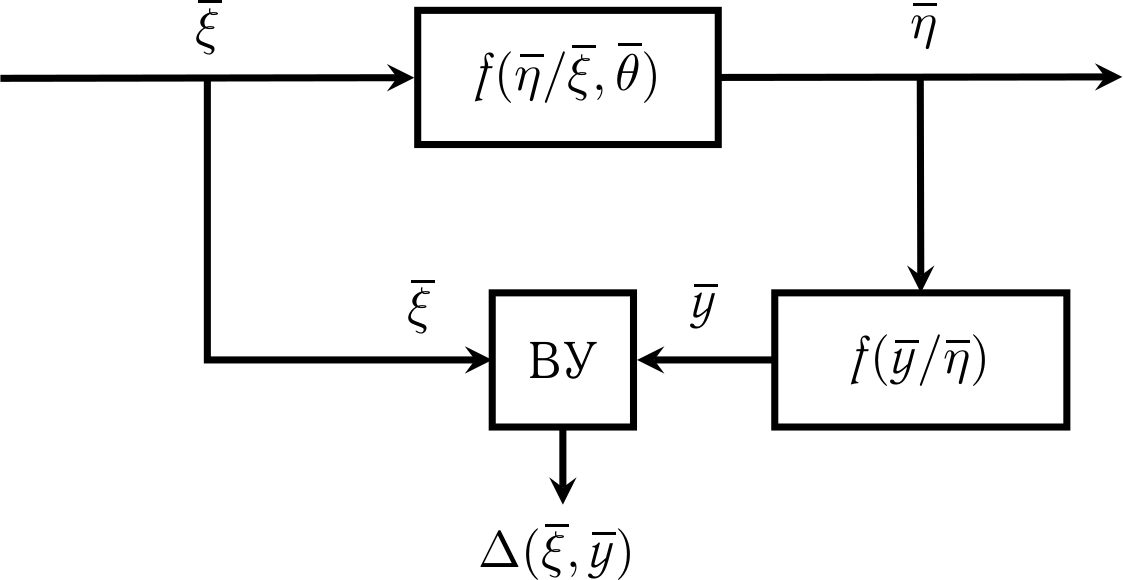
\includegraphics[width=100mm]{fig/half_new.png}
    }
    \caption{полустохастический объект}\label{fig:type_half}
  \end{subfigure}

  \vspace{2\baselineskip}
  \begin{subfigure}[b]{\linewidth}
    \centering
    \fcolorbox{gray}{white}{
      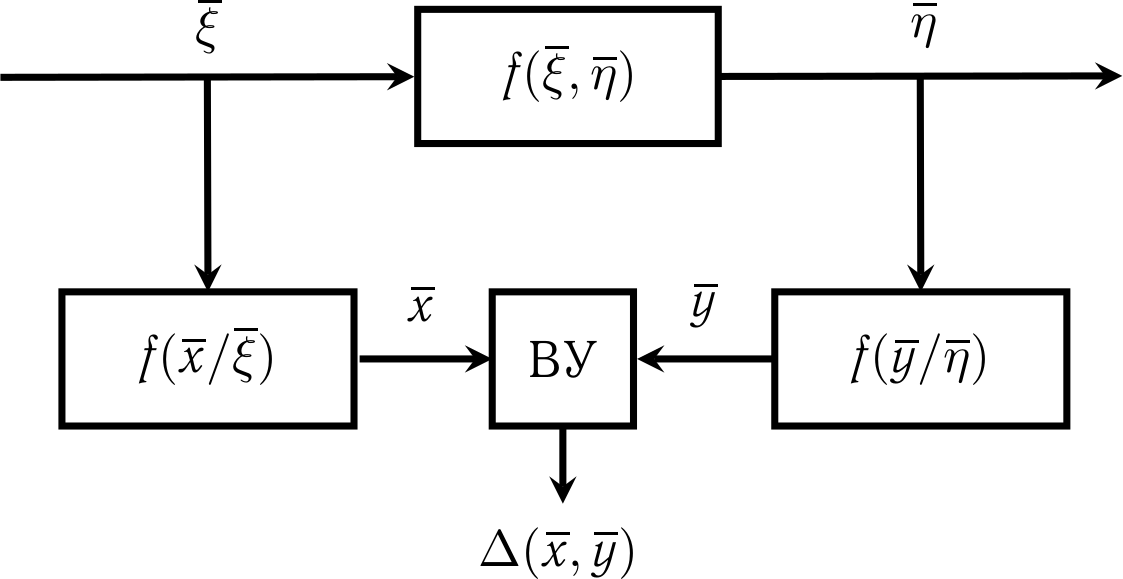
\includegraphics[width=100mm]{fig/first_new.png}
    }
    \caption{стохастический объект первого типа}\label{fig:type_first}
  \end{subfigure}

  \vspace{2\baselineskip}
  \begin{subfigure}[b]{\linewidth}
    \centering
    \fcolorbox{gray}{white}{
      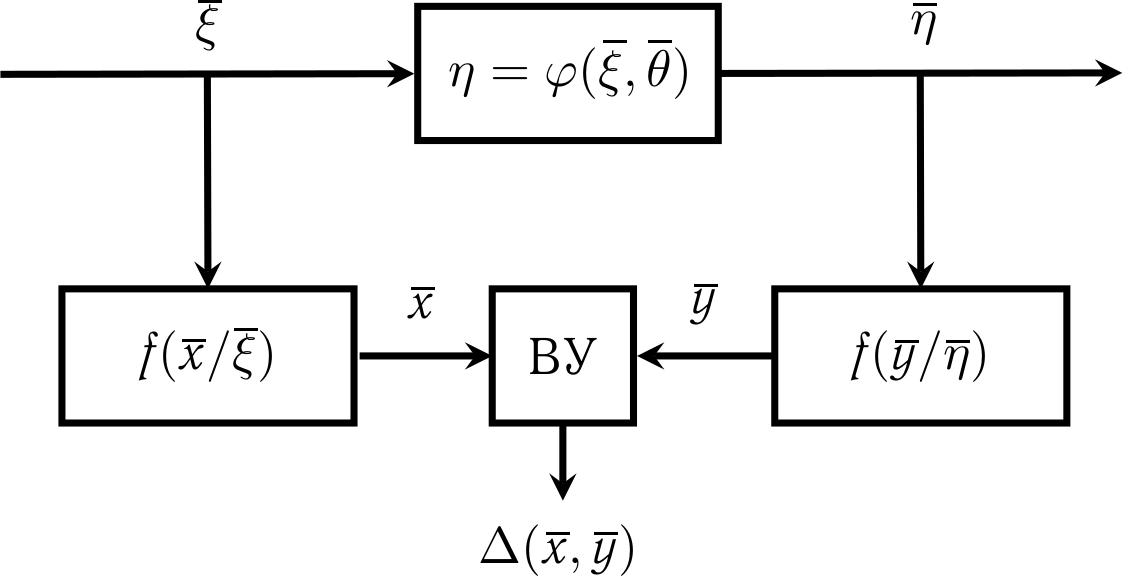
\includegraphics[width=100mm]{fig/second_new.png}
    }
    \caption{стохастический объект второго типа}\label{fig:type_second}
  \end{subfigure}

  \vspace{\baselineskip}
  \caption{Классификация стохастических объектов}
\end{figure}

\subsection{Критерии идентификации линейных стохастических систем}\label{ssec:state_criterion}

В настоящее время наиболее широкое распространение получил критерий
минимума суммы квадратов вертикальных расстояний \( \rho_{\text{к}_i} \)
от наблюдений выходной переменной до аппроксимирующей прямой или плоскости
(классический критерий наименьших квадратов, рисунок~\ref{fig:state_criteria_classic}).
Этот критерий формально применим ко всем типам рассмотренных в
подразделе~\ref{subsec:classification} объектов.

Наряду с этим, известен другой критерий, состоящий в минимизации суммы квадратов
перпендикулярных расстояний \( \rho_{\text{с}_i} \) от наблюдений входных и выходных переменных до
аппроксимирующей прямой или плоскости (симметричный критерий наименьших квадратов,
рисунок~\ref{fig:state_criteria_symmetric}).

\begin{figure}[h]
  \begin{subfigure}[b]{0.5\linewidth}
    \centering
    \fcolorbox{gray}{white}{
      % Graphic for TeX using PGF
% Title: /home/budnyjj/univer/magistracy/conferences/53/presentation/images/classic.dia
% Creator: Dia v0.97.3
% CreationDate: Tue May  2 14:01:26 2017
% For: budnyjj
% \usepackage{tikz}
% The following commands are not supported in PSTricks at present
% We define them conditionally, so when they are implemented,
% this pgf file will use them.
\ifx\du\undefined
  \newlength{\du}
\fi
\setlength{\du}{15\unitlength}
\begin{tikzpicture}
\pgftransformxscale{0.700000}
\pgftransformyscale{-0.700000}
\definecolor{dialinecolor}{rgb}{0.000000, 0.000000, 0.000000}
\pgfsetstrokecolor{dialinecolor}
\definecolor{dialinecolor}{rgb}{1.000000, 1.000000, 1.000000}
\pgfsetfillcolor{dialinecolor}
\pgfsetlinewidth{0.100000\du}
\pgfsetdash{}{0pt}
\pgfsetdash{}{0pt}
\pgfsetbuttcap
{
\definecolor{dialinecolor}{rgb}{0.000000, 0.000000, 0.000000}
\pgfsetfillcolor{dialinecolor}
% was here!!!
\pgfsetarrowsend{stealth}
\definecolor{dialinecolor}{rgb}{0.000000, 0.000000, 0.000000}
\pgfsetstrokecolor{dialinecolor}
\draw (15.950000\du,22.050000\du)--(16.000000\du,13.000000\du);
}
\pgfsetlinewidth{0.100000\du}
\pgfsetdash{}{0pt}
\pgfsetdash{}{0pt}
\pgfsetbuttcap
{
\definecolor{dialinecolor}{rgb}{0.000000, 0.000000, 0.000000}
\pgfsetfillcolor{dialinecolor}
% was here!!!
\pgfsetarrowsend{stealth}
\definecolor{dialinecolor}{rgb}{0.000000, 0.000000, 0.000000}
\pgfsetstrokecolor{dialinecolor}
\draw (15.000000\du,21.000000\du)--(28.000000\du,21.000000\du);
}
\pgfsetlinewidth{0.100000\du}
\pgfsetdash{}{0pt}
\pgfsetdash{}{0pt}
\pgfsetbuttcap
{
\definecolor{dialinecolor}{rgb}{0.000000, 0.000000, 0.000000}
\pgfsetfillcolor{dialinecolor}
% was here!!!
\definecolor{dialinecolor}{rgb}{0.000000, 0.000000, 0.000000}
\pgfsetstrokecolor{dialinecolor}
\draw (18.000000\du,14.000000\du)--(26.000000\du,20.000000\du);
}
\pgfsetlinewidth{0.100000\du}
\pgfsetdash{{1.000000\du}{1.000000\du}}{0\du}
\pgfsetdash{{0.600000\du}{0.600000\du}}{0\du}
\pgfsetbuttcap
{
\definecolor{dialinecolor}{rgb}{0.000000, 0.000000, 0.000000}
\pgfsetfillcolor{dialinecolor}
% was here!!!
}
\definecolor{dialinecolor}{rgb}{0.000000, 0.000000, 0.000000}
\pgfsetstrokecolor{dialinecolor}
\draw (20.000000\du,16.200000\du)--(20.000000\du,19.000000\du);
\pgfsetbuttcap
\pgfsetmiterjoin
\pgfsetdash{}{0pt}
\pgfsetlinewidth{0.100000\du}
\definecolor{dialinecolor}{rgb}{0.000000, 0.000000, 0.000000}
\pgfsetfillcolor{dialinecolor}
\pgfpathellipse{\pgfpoint{20.000000\du}{15.450000\du}}{\pgfpoint{0.250000\du}{0\du}}{\pgfpoint{0\du}{0.250000\du}}
\pgfusepath{fill}
\definecolor{dialinecolor}{rgb}{0.000000, 0.000000, 0.000000}
\pgfsetfillcolor{dialinecolor}
\fill (20.250000\du,16.200000\du)--(20.000000\du,15.700000\du)--(19.750000\du,16.200000\du)--cycle;
\pgfsetbuttcap
\pgfsetmiterjoin
\pgfsetdash{}{0pt}
\pgfsetlinewidth{0.100000\du}
\definecolor{dialinecolor}{rgb}{0.000000, 0.000000, 0.000000}
\pgfsetfillcolor{dialinecolor}
\pgfpathellipse{\pgfpoint{20.000000\du}{19.750000\du}}{\pgfpoint{0.250000\du}{0\du}}{\pgfpoint{0\du}{0.250000\du}}
\pgfusepath{fill}
\definecolor{dialinecolor}{rgb}{0.000000, 0.000000, 0.000000}
\pgfsetfillcolor{dialinecolor}
\fill (19.750000\du,19.000000\du)--(20.000000\du,19.500000\du)--(20.250000\du,19.000000\du)--cycle;
% setfont left to latex
\definecolor{dialinecolor}{rgb}{0.000000, 0.000000, 0.000000}
\pgfsetstrokecolor{dialinecolor}
\node[anchor=west] at (18.000000\du,17.800000\du){$ \rho_{\text{к}_i} $};
% setfont left to latex
\definecolor{dialinecolor}{rgb}{0.000000, 0.000000, 0.000000}
\pgfsetstrokecolor{dialinecolor}
\node[anchor=west] at (20.300000\du,20.000000\du){$ (x_i, y_i) $};
% setfont left to latex
\definecolor{dialinecolor}{rgb}{0.000000, 0.000000, 0.000000}
\pgfsetstrokecolor{dialinecolor}
\node[anchor=west] at (18.500000\du,20.000000\du){};
% setfont left to latex
\definecolor{dialinecolor}{rgb}{0.000000, 0.000000, 0.000000}
\pgfsetstrokecolor{dialinecolor}
\node[anchor=west] at (20.300000\du,15.000000\du){$ (x_i, \hat{\alpha}_{\text{к}} + \hat{\beta}_{\text{к}} x_i ) $};
\end{tikzpicture}

    }
    \caption{классический}\label{fig:state_criteria_classic}
  \end{subfigure}
  \hfill
  \begin{subfigure}[b]{0.5\linewidth}
    \centering
    \fcolorbox{gray}{white}{
      % Graphic for TeX using PGF
% Title: /home/budnyjj/univer/magistracy/conferences/53/presentation/images/symmetric.dia
% Creator: Dia v0.97.3
% CreationDate: Tue May  2 14:15:14 2017
% For: budnyjj
% \usepackage{tikz}
% The following commands are not supported in PSTricks at present
% We define them conditionally, so when they are implemented,
% this pgf file will use them.
\ifx\du\undefined
  \newlength{\du}
\fi
\setlength{\du}{15\unitlength}
\begin{tikzpicture}
\pgftransformxscale{0.700000}
\pgftransformyscale{-0.700000}
\definecolor{dialinecolor}{rgb}{0.000000, 0.000000, 0.000000}
\pgfsetstrokecolor{dialinecolor}
\definecolor{dialinecolor}{rgb}{1.000000, 1.000000, 1.000000}
\pgfsetfillcolor{dialinecolor}
\pgfsetlinewidth{0.100000\du}
\pgfsetdash{}{0pt}
\pgfsetdash{}{0pt}
\pgfsetbuttcap
{
\definecolor{dialinecolor}{rgb}{0.000000, 0.000000, 0.000000}
\pgfsetfillcolor{dialinecolor}
% was here!!!
\pgfsetarrowsend{stealth}
\definecolor{dialinecolor}{rgb}{0.000000, 0.000000, 0.000000}
\pgfsetstrokecolor{dialinecolor}
\draw (15.950000\du,22.050000\du)--(16.000000\du,13.000000\du);
}
\pgfsetlinewidth{0.100000\du}
\pgfsetdash{}{0pt}
\pgfsetdash{}{0pt}
\pgfsetbuttcap
{
\definecolor{dialinecolor}{rgb}{0.000000, 0.000000, 0.000000}
\pgfsetfillcolor{dialinecolor}
% was here!!!
\pgfsetarrowsend{stealth}
\definecolor{dialinecolor}{rgb}{0.000000, 0.000000, 0.000000}
\pgfsetstrokecolor{dialinecolor}
\draw (15.000000\du,21.000000\du)--(28.000000\du,21.000000\du);
}
\pgfsetlinewidth{0.100000\du}
\pgfsetdash{}{0pt}
\pgfsetdash{}{0pt}
\pgfsetbuttcap
{
\definecolor{dialinecolor}{rgb}{0.000000, 0.000000, 0.000000}
\pgfsetfillcolor{dialinecolor}
% was here!!!
\definecolor{dialinecolor}{rgb}{0.000000, 0.000000, 0.000000}
\pgfsetstrokecolor{dialinecolor}
\draw (17.006017\du,14.015552\du)--(26.000000\du,18.000000\du);
}
\pgfsetlinewidth{0.100000\du}
\pgfsetdash{{1.000000\du}{1.000000\du}}{0\du}
\pgfsetdash{{0.600000\du}{0.600000\du}}{0\du}
\pgfsetbuttcap
{
\definecolor{dialinecolor}{rgb}{0.000000, 0.000000, 0.000000}
\pgfsetfillcolor{dialinecolor}
% was here!!!
}
\definecolor{dialinecolor}{rgb}{0.000000, 0.000000, 0.000000}
\pgfsetstrokecolor{dialinecolor}
\draw (21.552786\du,16.894427\du)--(20.447214\du,19.105573\du);
\pgfsetbuttcap
\pgfsetmiterjoin
\pgfsetdash{}{0pt}
\pgfsetlinewidth{0.100000\du}
\definecolor{dialinecolor}{rgb}{0.000000, 0.000000, 0.000000}
\pgfsetfillcolor{dialinecolor}
\pgfpathellipse{\pgfpoint{21.888197\du}{16.223607\du}}{\pgfpoint{0.250000\du}{0\du}}{\pgfpoint{0\du}{0.250000\du}}
\pgfusepath{fill}
\pgfpathellipse{\pgfpoint{20.111803\du}{15.3923607\du}}{\pgfpoint{0.250000\du}{0\du}}{\pgfpoint{0\du}{0.250000\du}}
\pgfusepath{fill}
\definecolor{dialinecolor}{rgb}{0.000000, 0.000000, 0.000000}
\pgfsetfillcolor{dialinecolor}
\fill (21.776393\du,17.006231\du)--(21.776393\du,16.447214\du)--(21.329180\du,16.782624\du)--cycle;
\pgfsetbuttcap
\pgfsetmiterjoin
\pgfsetdash{}{0pt}
\pgfsetlinewidth{0.100000\du}
\definecolor{dialinecolor}{rgb}{0.000000, 0.000000, 0.000000}
\pgfsetfillcolor{dialinecolor}
\pgfpathellipse{\pgfpoint{20.111803\du}{19.776393\du}}{\pgfpoint{0.250000\du}{0\du}}{\pgfpoint{0\du}{0.250000\du}}
\pgfusepath{fill}
\definecolor{dialinecolor}{rgb}{0.000000, 0.000000, 0.000000}
\pgfsetfillcolor{dialinecolor}
\fill (20.223607\du,18.993769\du)--(20.223607\du,19.552786\du)--(20.670820\du,19.217376\du)--cycle;
% setfont left to latex
\definecolor{dialinecolor}{rgb}{0.000000, 0.000000, 0.000000}
\pgfsetstrokecolor{dialinecolor}
\node[anchor=west] at (18.500000\du,18.000000\du){$ \rho_{\text{с}_i} $};
% setfont left to latex
\definecolor{dialinecolor}{rgb}{0.000000, 0.000000, 0.000000}
\pgfsetstrokecolor{dialinecolor}
\node[anchor=west] at (20.300000\du,20.000000\du){$ (x_i, y_i) $};
% setfont left to latex
\definecolor{dialinecolor}{rgb}{0.000000, 0.000000, 0.000000}
\pgfsetstrokecolor{dialinecolor}
\node[anchor=west] at (18.500000\du,20.000000\du){};
% setfont left to latex
\definecolor{dialinecolor}{rgb}{0.000000, 0.000000, 0.000000}
\pgfsetstrokecolor{dialinecolor}
\node[anchor=west] at (20.300000\du,14.700000\du){$ (x_i, \psi(\hat{\theta_{\text{с}}}, x_i)) $};
\end{tikzpicture}

    % $ \varepsilon = N(0, \sigma_{\varepsilon}), \delta = N(0, \sigma_{\delta}) $
    % --- ошибки измерений, \\

    }
    \caption{симметричный}\label{fig:state_criteria_symmetric}
  \end{subfigure}

  \vspace{\baselineskip}
  \caption{Критерии идентификации стохастических систем}
\end{figure}

Данный критерий был предложен К.~Пирсоном в статье~\cite{pearson_1901}
для линейной аппроксимации стохастических объектов первого и второго типов.
Решение, полученное К.~Пирсоном, характеризуется скалярным подходом и
представляется неудобным для использования.
В связи с этим в работе~\cite{mukha_2016} было получено независимое решение задачи с
указанным критерием в векторно-матричной форме.
Вопрос области применения этой аппроксимации является открытым.

Известно, что задача линейной аппроксимации полустохастического объекта полностью решена в
рамках классического линейного регрессионного анализа как задача оценивания параметров
линейной математической модели объекта с критерием минимизации суммы квадратов вертикальных расстояний.
Оптимальное решение здесь "--- классическая линейная регрессия,
обеспечивающая как оптимальное оценивание параметров математической модели объекта
(при заданных значениях входных переменных),
так и оптимальное прогнозирование наблюдений выходных переменных по наблюдениям входных переменных.

Ввиду того, что стохастический объект первого типа не имеет реальных параметров,
сравнение точности оценивания его параметров лишено смысла.
В работах~\cite{mukha_2010, mukha_2011} была сформулирована задача оптимального прогнозирования
выходных переменных линейного стохастического объекта первого типа и показано,
что оптимальным линейным предиктором также является классическая линейная регрессия.

Относительно стохастического объекта второго типа следует отметить,
что области предпочтительного использования классического и симметричного критериев
определены недостаточно четко.
Выявление условий предпочтительного использования этих критериев входит в задачи данной работы.

\vspace{2\baselineskip}
\subsection{Идентификация нелинейных стохастических систем}\label{ssec:state_nonlinear}

Оптимальному оцениванию параметров детерминированного объекта по измерениям с ошибками
посвящен ряд работ, обзор которых имеется в статье~\cite{fedorov_1978}.
Полученные к настоящему времени решения представляют собой, как правило,
состоятельные итерационные процедуры.
Однако существующие исследования нельзя считать достаточно завершенными:
отсутствует обоснование используемых критериев,
не приводится сравнительный численный анализ различных алгоритмов,
отсутствуют рекомендации по применению того или иного алгоритма.
Представляется целесообразной попытка независимого решения этой задачи.

\vspace{2\baselineskip}
\section{Постановка задачи исследования}

Требуется выполнить численный сравнительный анализ точности
методов идентификации стохастических систем второго типа.
На основании полученных результатов необходимо описать
условия предпочтительного использования сравниваемых методов
для оценивания параметров систем.

\section{Выводы}

\begin{enumerate}
\item Выполнен анализ задач и критериев идентификации стохастических систем.
\item Предложена классификация стохастических объектов для целей
  идентификации и сравнения.
\end{enumerate}